\subsection{Story Mapping}
\blockquote{We spend lots of time working with our customers. We work hard to understand their goals, their users, and the major parts of the system we could build. Then we finally get down to the details - the pieces of functionality we'd like to build. In my head a see a tree where the trunk is built from the goals or desired benefits that drive the system; big branches are users; the small branches and twigs are the capabilities they need; then finally the leaves are the user stories small enough to place into development iterations.

After all that work, after establishing all that shared understanding I feel like we pull all the leaves off the tree and load them into a leaf bag - then cut down the tree.

That's what a flat backlog is to me. A bag of context-free mulch.

I need that context in order for me to really tell a story about the system.

-- Jeff Patton
}

Story Map Structure: Goals > Activities > Tasks > Stories

\begin{figure}[H] % Example image
\center{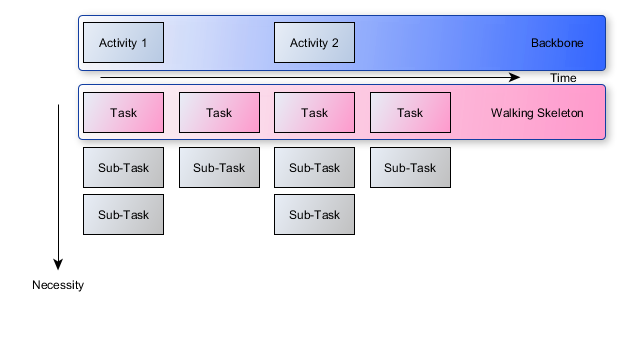
\includegraphics[width=1\linewidth]{RE/StoryMap}}
\caption{Story Map Pattern}
\label{fig:re:storymap}
\end{figure}

\blockquote{When arranging stories in the map, if a person using the system typically does one thing after another, then I'll put the early thing on the left, and the later thing on the right. I do this with the big things and the little things - the activities and the tasks.

When teaching this, people often tell me "the users can perform these in any order. What order should I put them in?" I'll ask them to "explain to me what the system does at a high level - just tell me the activities." They then recite them to me. "That's the order" I say. In fact, the order you'd explain the behavior of the system in is the correct order. We're building a map that lets us tell a really big story about the system. Build the map in a way that helps you tell the story.}

\blockquote{When it's time to plan releases, it's usually not important to prioritize backbone items against each other. For instance if I were to build a high level backlog for a car it might look something like this: engine, transmission, brakes, suspension, etc.

It would be stupid to ask stakeholders to prioritize that: "what's more important, the engine or the transmission?" or "we don't have enough time in this release, could we release without brakes and add them later?" These items are essential - and we'll need all of them to deliver a minimum viable product - and MVP.

Where the prioritization comes in is below this level: 4-cylinder engine or 6-cylinder engine? brakes with anti-locking or brakes without? sport suspension or not? It's how we build up those backbone items - prioritize their characteristics that matters.

When you prioritize a story map, you'll move cards or stickies up and down to indicate high or low. Lately I take a long strip of masking tape and line off the story map - creating horizontal swim lanes for each release. Then I move the stories up and down into each lane, and even vary their height in the lane.}

